\section{Metodologia testowania}
\subsection{Warunki testowe i zastosowane środki bezpieczeństwa}
Ze względu na mój relatywny brak doświadczenia w sferze cyberbezpieczeństwa postanowiłem 
zachować możliwie największe środki ostrożności podczas wykonywania scenariuszy ataku. W szczególności tyczy się to infekcji prawdziwym wirusem ransomware.\newline
Moim stanowiskiem pracy był laptop Asus TUF Gaming FX505D~z~8 GB ramu i 512 GB pamięci NVME~z~zainstalowanym Linuksem Proxmox VE 8.1\footnote{Obraz systemu został pobrany ze strony \url{https://www.proxmox.com/en/downloads}. SHA256 obrazu wynosiło 9018a17307ad50eb9bf32a805d0917d621499363ef87b0b477332ed9f9d7dcc1.}. Proxmox jest dystrybucją specjalizującą się w zarządzaniu wirtualną infrastrukturą (na rodzaj VmWare). Posiada ona wygodny interfejs graficzny dostępny przez sieć oraz wiele udogodnień z dziedziny wirtualizacji.
\newline
Wszystkie testowane maszyny wirtualne mają zainstalowanego Ubuntu Server 22.04 LTS\footnote{\url{https://ubuntu.com/download/server}}. Każda z wirtualnych maszyn ma przydzielone 32 GB pamięci twardej, 8GB pamięci RAM oraz 8 procesorów. Jako hypervisor korzystałem~z~QEMU\footnote{\url{https://www.qemu.org/}} bez KVM\footnote{\url{https://linux-kvm.org/page/Main_Page}}.
Mimo iż użycie KVM przyspieszyłoby działanie maszyn wirtualnych, postanowiłem~z~niego nie korzystać z~powodu braku konkretnych dowodów na absolutną odporność KVM switcha na oprogramowanie złośliwe. Dodatkowym środkiem bezpieczeństwa było zupełne wyizolowanie wirtualnych maszyn we własnych podsieciach na maszynie, która sama także była kompletnie fizycznie odizolowana od sieci zewnętrznych. Zasady audytu na maszynach zostały utworzone w trybie \foreignquote{english}{immutable}, tym samym nie mogły zostać zmienione bez ponownego uruchomienia systemu.
\begin{figure}[H]
    \centering
    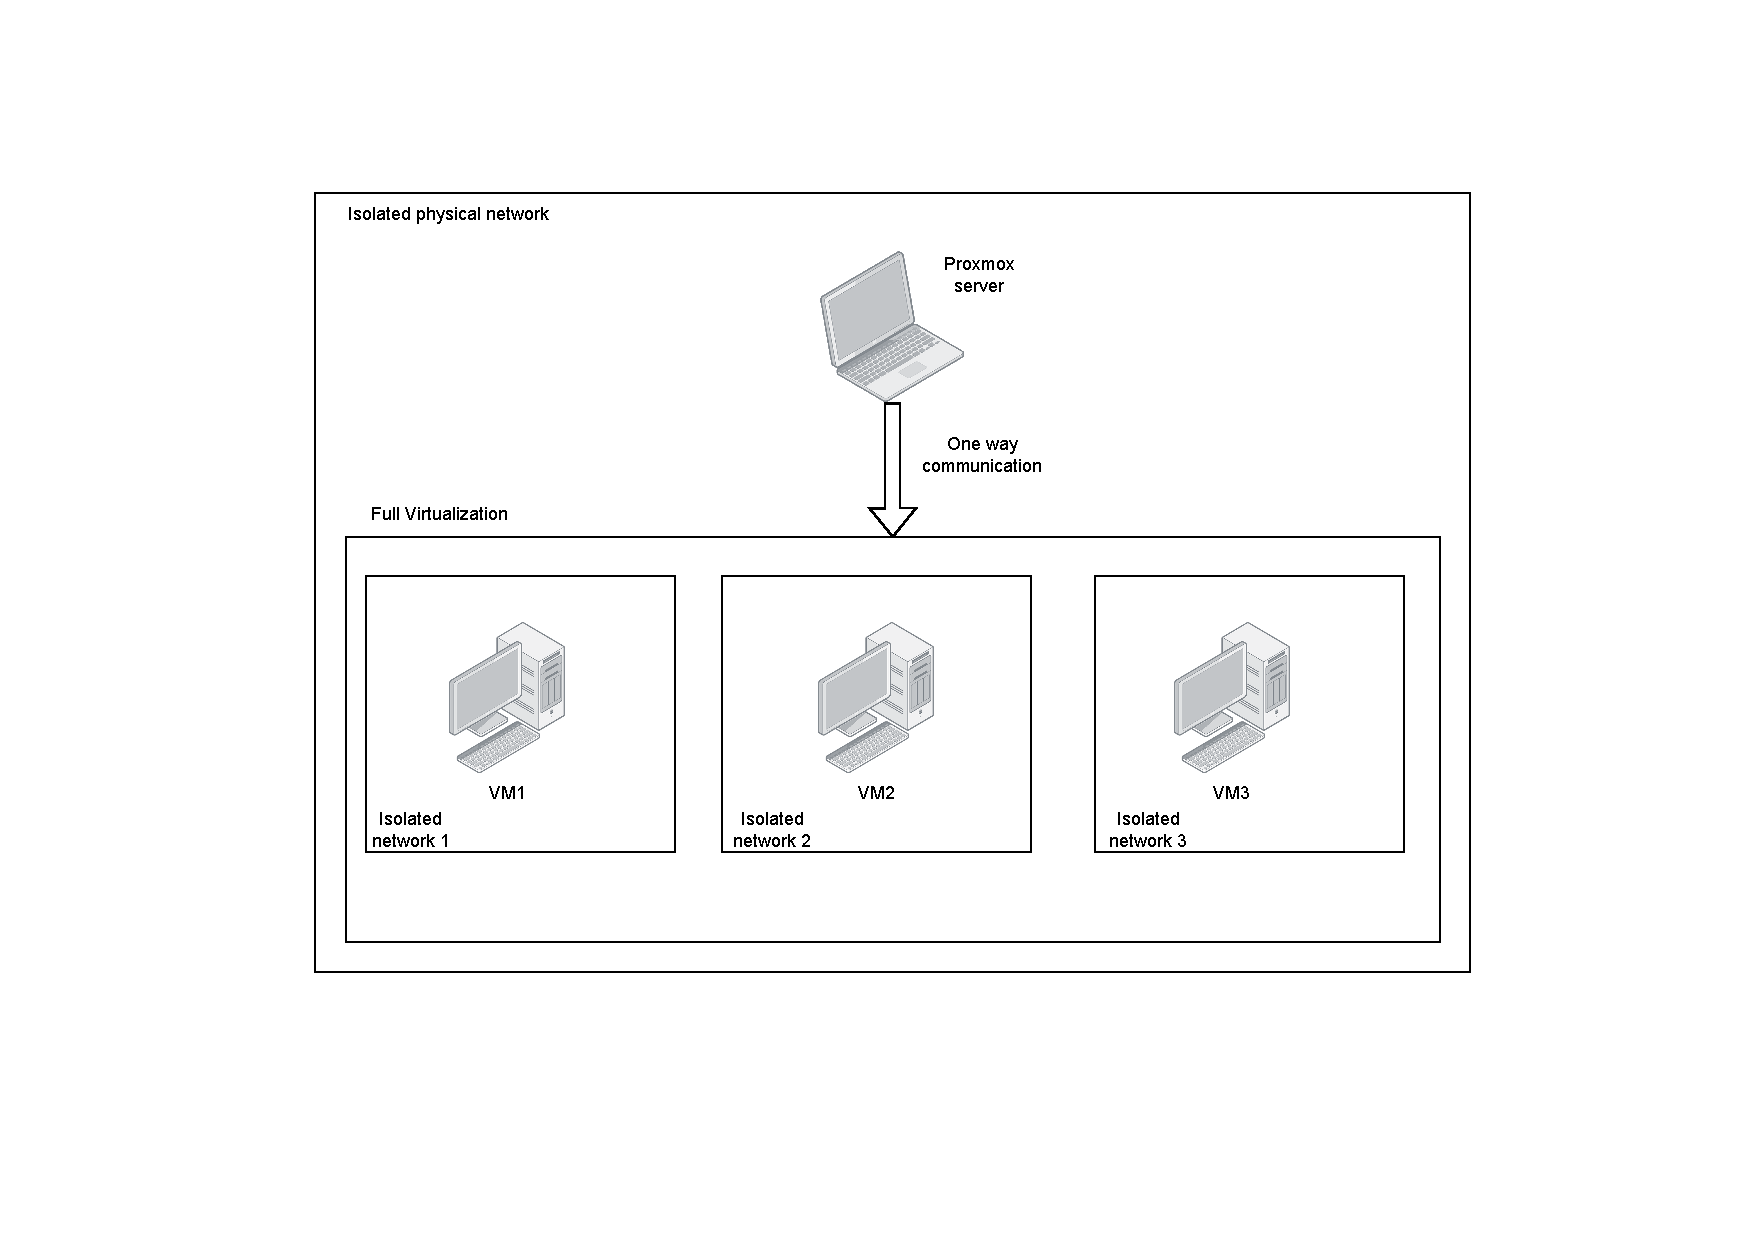
\includegraphics[width=0.8\linewidth]{rysunki/test.drawio.pdf}
    \caption{Architektura infrastruktury testowej.}
    \label{fig:enter-label}
\end{figure}

\subsection{Ustalenie metryki skuteczności rozwiązania}
Podstawowym założeniem testów była pewność odbywania się ataku podczas działania aplikacji. W tym wypadku nie ma sensu testowanie skuteczności w formie wartości dokładności wykrywania obecności ataku, gdyż jest on stałym elementem wszystkich scenariuszy. Zamiast tego postanowiłem, że skuteczność rozwiązania będzie mierzona na podstawie \emph{czasu wykrycia} od momentu rozpoczęcia ataku. Jest to miarodajna metryka naturalnie powiązanya~z~potencjalnym zakresem strat w organizacji zagrożonej ransomware.
\newline
Niestety średni czas wykrycia ataku według raportu IBMu w 2018 roku wyniósł 197 dni, a w 2019 - 207 dni~\cite{security_2019_nodate}. Aby test był możliwy do wykonania w sensownym terminie, zmuszony byłem skrócić jego czas. W związku z tym postanowiłem obrać subiektywnie wybraną miarę, umotywowaną niewielkim rozmiarem systemów użytych w testach. Mianowicie - \textbf{jeśli na 10 godzin od rozpoczęcia ataku zostanie wykryte potencjalne zagrożenie, to test został zakończony sukcesem} w przeciwnym wypadku dojdzie do porażki. W ramach testu aplikacja będzie aktywna w tle jeszcze przed rozpoczęciem ataku.
%%%%%%%%%%%%%%%%%%%%%%%%%%%%%%%%%%%%%%%%%%%%%%%%%%%%%%%%%%%%%%%%%%%%%%%%%%%%%%%%%%%%
\section{Scenariusze testowe symulujące ataki ransomware}
\subsection{Improwizowany atak~z~kompresowaniem}
Jako podstawowy scenariusz postanowiłem dokonać ataku za pomocą archiwizacji~z~szyfrowaniem w folderze~z~milionem plików. Atak miał na celu zaszyfrowanie wyłącznie plików~z~rozszerzeniem \texttt{.txt}. W tym samym miejscu obecne były również pliki o innych rozszerzeniach.
\begin{lstlisting}[language=bash,
    backgroundcolor=\color{EEGold!5!white},
    caption={Komenda użyta do wykonania "ataku".},
    label={lst:commau}]
    $ zip --encrypt files.zip *.txt
    $ rm -f *.txt
\end{lstlisting}
Warto dodać, że komenda nie wymagała przywilejów super usera. Istnieje więc możliwość wystąpienia podobnego ataku w organizacji w której doszło do wycieku danych kont pracowników bez przywilejów sudo.
\begin{lstlisting}[language=bash,
    backgroundcolor=\color{EEGold!5!white},
    caption={Fragment logów~z~komponentu zbierającego informacje o systemie plików.},
    label={lst:logau}]
    2023-12-17T22:33:07.316 z INFO Inserting {"user":"userA","group":"userA","executable":"/usr/bin/rm","syscall":"unlinkat","timestamp":"1702852387","key":"WRITE"}
    2023-12-17T22:33:07.351 z WARN Blocking error while reading from socket
    2023-12-17T22:33:09.762 z INFO Unix stream is readable.
    2023-12-17T22:33:09.762 z INFO Opening an Sqlite connection
    2023-12-17T22:33:09.763 z INFO Inserting {"user":"userA","group":"userA","executable":"/usr/bin/bash","syscall":"openat","timestamp":"1702852389","key":"READ"}
    2023-12-17T22:33:09.781 z INFO Opening an Sqlite connection
    2023-12-17T22:33:09.792 z WARN Blocking error while reading from socket
    2023-12-17T22:33:12.999 z INFO Unix stream is readable
    2023-12-17T22:33:12.999 z INFO Opening an Sqlite connection
    2023-12-17T22:33:12.999 z INFO Inserting {"user":"userA","group":"userA","executable":"/usr/bin/zip","syscall":"openat","timestamp":"1702852392","key":"WRITE"}
    2023-12-17T22:33:13.028 z INFO Opening an Sqlite connection
    2023-12-17T22:33:13.053 z INFO Unix stream is readable.
    2023-12-17T22:33:13.053 z INFO Opening an Sqlite connection
    2023-12-17T22:33:13.053 z INFO Inserting {"user":"userA","group":"userA","executable":"/usr/bin/zip","syscall":"unlink","timestamp":"1702852393","key":"WRITE"}
    2023-12-17T22:33:13.100 z INFO Opening an Sqlite connection
\end{lstlisting}
Logi~z~części aplikacji związanej ze zbieraniem informacji o systemie plików treściwie ukazują zakres działania tego komponentu. W trybie informacyjnym można zauważyć przewijanie się linijek~z~informacjami~o~odczytanych operacjach. Dodatkowo można zauważyć status odczytu~z~gniazda \texttt{auditd} oraz informacje~o~zapisie danych~o~operacji do bazy SQLite.\newpage

\begin{lstlisting}[language=bash,
    backgroundcolor=\color{EEGold!5!white},
    caption={Raport wygenerowany ze skanera, który pozwoliłem sobie delikatnie sformatować aby widać było lepiej jego treść.},
    label={lst:raportau}]
    <9>1 2023-12-18T18:11:20.485Z
    test-hostname 
    ransomware-scanner 
    - - -  
Strategy evaluations: {
    "Executable":"Low",
    "Threshold":"High",
    "Rename":"Low",
    "RansomNote":"Low"}
File risk evaluation {
    "/home/userA/box/testfile.png":"Medium",
    "/home/userA/box/h1.csv":"Low",
    "/home/userA/box/files.zip":"High",
    "/home/userA/box/h2.csv":"Low"}
\end{lstlisting}
W raporcie \enquote{z~autopsji} można zobaczyć, że jedyną metodą, która wykryła podejrzany ruch na maszynie była strategia~z~przekroczeniem ustalonej ilości operacji na jednostkę czasu. W wypadku tej maszyny było to 300 operacji na 100 ms. 
Czas wykrycia pokrył się~z~interwałem inicjalizacji analizy i wyniósł ok \textbf{167 ms}.
\newline
We fragmencie zatytułowanym \foreignquote{english}{File risk evaluation} każdy plik określony swoją absolutną ścieżką ma ustaloną wartość ewaluacji. Dla plików wykonywalnych oznacza to jak wysokie jest ryzyko tego, że program jest oprogramowaniem złośliwym. Dla wszystkich innych rodzajów plików wyznaczone jest ryzyko zaszyfrowania go. Jak widać plik \texttt{files.zip} jako jedyny został oznaczony jako plik wysokiego ryzyka bycia zaszyfrowanym.

\subsection{Atak Ransom EXX}
W drugim scenariuszu dokonałem na maszynie testowej ataku wirusem Ransom EXX. Scenariusz zakłada użycie \textbf{prawdziwego} wariantu wirusa\footnote{Na własną odpowiedzialność można go zdobyć ze strony \url{https://github.com/Gi7w0rm/RansomExx_samples_and_related_artifacts}}. Próbka którą wykorzystałem ma wartość funkcji SHA-256 równą 196eb5bfd52d4a538d4d0a801808298faadec1fc9aeb07c231add0161b416807. Wirus w tej wersji to plik wykonywalny (ELF) którego ciekawymi aspektami jest brak sekcji \texttt{.note.gnu.build-id}~o~której była mowa w sekcji \hyperref[sec:elfini]{Krótka charakterystyka plików wykonywalnych}. Postawiona przeze mnie w tamtej sekcji propozycja częściowej identyfikacji plików wykonywalnych poprzez analizę ich nagłówka miała tutaj swoje ograniczone zastosowanie. Zanim rozpocząłem atak, umieściłem w ścieżce instalacyjnej skanera wydzieloną część \texttt{.data} wirusa~z~wariantu~o~SHA-256 równym aa1ddf0c8312349be614ff43e80a262f, aby program mógł skorzystać~z~niej przy liczeniu podobieństwa cosinusowego. Atak został wywołany~z~obserwowanej ścieżki, której prefixem jest \texttt{/home}.

\begin{lstlisting}[language=bash,
    backgroundcolor=\color{EEGold!5!white},
    caption={Pierwszy raport~z~ataku Ransom EXX.},
    label={lst:raportau}]
    <9>1 2023-12-19T18:28:55.009Z
    test-hostname 
    ransomware-scanner 
    - - -  
Strategy evaluations: {
    "Rename":"Low",
    "Threshold":"Low",
    "Executable":"High",
    "RansomNote":"Low"}
File risk evaluation {
    "/home/userA/box/documentFile.txt":"Low",
    "/home/userA/box/testfile.png":"Low",
    "/home/userA/box/h1.csv":"Low",
    "/home/userA/box/h2.csv":"Low"
    "/home/maciek/box/exx196":"High"}
\end{lstlisting}
Zanim plik wykonywalny został aktywowany, jego obecność została oznaczona jako ryzykowna. Można więc powiedzieć, że test został zakończony sukcesem. Mimo to pozostawiłem maszynę do następnego dnia. Co ciekawe wg. raportu w czasie 16 godzin od rozpoczęcia ataku żaden~z~plików w \texttt{/home} nie został zaszyfrowany.
Reguły audytowania nie zostały naruszone, podobnie żaden~z~komponentów aplikacji. Dodatkowo pliki, które widać w raporcie posiadają rozszerzenia formatów będących typowym celem ataków. Jest to prawdopodobnie spowodowane powolnym działaniem wirusa.  Mimo to, podejście polegające na wykrywaniu \enquote{podejrzanych} plików i plików zaszyfrowanych znalazło tu swoje zastosowanie.
\begin{lstlisting}[language=bash,
    backgroundcolor=\color{EEGold!5!white},
    caption={Drugi raport~z~ataku Ransom EXX.},
    label={lst:raportau}]
    <9>1 2023-12-20T10:40:13.344Z
    test-hostname 
    ransomware-scanner 
    - - -  
Strategy evaluations: {
    "Rename":"Low",
    "Threshold":"Low",
    "Executable":"High",
    "RansomNote":"Low"}
File risk evaluation {
    "/home/userA/box/documentFile.txt":"Low",
    "/home/userA/box/testfile.png":"Low",
    "/home/userA/box/h1.csv":"Low",
    "/home/userA/box/h2.csv":"Low"
    "/home/maciek/box/exx196":"High"}
\end{lstlisting}
%
% Log~z~autopsji
% no bo została wykryta binarka, prawdopodobnie nie można 
%
\subsection{Atak Hive}
Hive jest wirusem występującym zarówno w wariancie Windowsowym 
jak i Linuksowym. 
Wersja Linuksowa została specjalnie stworzona pod atak infrastruktury wirtualnej, między 
innymi infekcję maszyn wirtualnych. Do ciekawych aspektów tego wirusa należy fakt napisania go w języku GO oraz to, że jego wersja Linuksowa wedle doniesień posiada wiele błędów~i~niedociągnieć. W trakcie testu napotkałem kilka~z~nich, między innymi błąd braku możliwości rozpoczęcia programu jeśli jest on wywołany wraz~z~prefixem ścieżki (bez znaczenia czy relatywnej czy absolutnej).
Próbka którą wykorzystałem ma wartość funkcji SHA-256 równą
713b699c04f21000fca981e698e1046d4595f423bd5741d712fd7e0bc358c771\footnote{Zdobyta ze strony: \url{https://bazaar.abuse.ch/sample/713b699c04f21000fca981e698e1046d4595f423bd5741d712fd7e0bc358c771/}}. Podobnie jak wirus~z~poprzedniej sekcji, występuje on w formacie ELF, lecz w przeciwieństwie do niego, posiada identyfikator kompilacji. Prawdopodobnie wynika to~z~domyślnych ustawień kompilatora GO. Również i tu wydzieliłem sekcję \texttt{.data} w celu skojarzenia podobieństwa plików wykonywalnych, ale tym razem niestety musiałem skorzystać z treści testowanego wirusa zamiast pochodnej ze względu na brak próbek. Atak został wywołany~z~obserwowanej ścieżki, której prefixem jest \texttt{/home}. Podobnie jak w porzednim scenariuszu, wirus został wykryty poprzez podobieństwo plików wykonywalnych. Z~tego powodu pozostawiłem maszynę wraz z działającym na nim wirusem na okres 10 godzin.
\begin{lstlisting}[language=bash,
    backgroundcolor=\color{EEGold!5!white},
    caption={Późniejszy raport~z~ataku Hive.},
    label={lst:raportau}]
    <9>1 2023-12-20T16:16:29.564Z
    test-hostname 
    ransomware-scanner 
    - - -  
Strategy evaluations: {
    "Rename":"Low",
    "Threshold":"Low",
    "Executable":"High",
    "RansomNote":"High"}
File risk evaluation {
    "/home/userA/box/HOW-TO-DECRYPT.txt": "High",
    "/home/userA/box/documentFile.txt":"Low",
    "/home/userA/box/testfile.png":"Low",
    "/home/userA/box/h1.csv":"Low",
    "/home/userA/box/h2.csv":"Low"
    "/home/maciek/box/hive":"High"}
\end{lstlisting}
Wyniki były zaskakujące. Według raportu, żaden~z~plików nie został zaszyfrowany. W obserwowanym folderze pojawił się plik \foreignquote{english}{HOW-TO-DECRYPT.txt} oceniony metodą wykrywania wiadomości~o~okupie jako niebezpieczny. W raporcie można także wyczytać, że wirus został wykryty metodą podobieństwa cosinusowego~o~czym wspomniałem wcześniej.\newpage
\begin{lstlisting}[
    backgroundcolor=\color{EEGold!5!white},
    caption={Fragment wiadomości~o~okupie. Ze względów bezpieczeństwa usunąłem wszelkie linki, loginy i hasła~z~listingu.},
    label={lst:raportau}]
    Your network has been breached and all data is encrypted.
    To decrypt all the data you will need to purchase our decryption software.
    Please contact our sales department at:
    <url>
    Login: <login>
    Password: <password>
    Follow the guidelines below to avoid losing your data:
    - Do not shutdown or reboot your computers, unmount external storages.
    - Do not try to decrypt data using third party software. It may cause irreversible damage.
\end{lstlisting}
Po dokładnym sprawdzeniu systemu plików na maszynie nie znalazłem żadnych śladów działania wirusa. Zasady audytu również nie zostały naruszone. Mimo dużej ilości informacji~o~błędach Linuksowej odmiany tego wirusa, nie byłem w stanie ustalić jednoznacznie dlaczego oprogramowanie wygenerowało dopiero po ok. 6 godzinach informacje~o~okupie bez~wyrządzenia widocznej szkody na systemie plików. Istnieje równa szansa, że może być to zarówno błąd oprogramowania jak i zamierzony cel (choć bardzo dziwny).

%\section{Analiza działań systemu~i~statystyk generowanych podczas symulowanego ataku}
\section{Ewaluacja skuteczności wykrywania}

\begin{table}[H]
    \centering
    \begin{tabular}{|l|l|l|l|l|}
    \hline
    Scenariusz\textbackslash{}Strategia wykrycia & Rename                      & Threshold                    & Executable                   & Ransom Note                  \\ \hline
    Improwizowany atak~z~kompresowaniem          & \cellcolor[HTML]{FD6864}Low & \cellcolor[HTML]{9AFF99}High & \cellcolor[HTML]{FD6864}Low  & \cellcolor[HTML]{FD6864}Low  \\ \hline
    Ransom EXX                                   & \cellcolor[HTML]{FD6864}Low & \cellcolor[HTML]{FD6864}Low  & \cellcolor[HTML]{67FD9A}High & \cellcolor[HTML]{FD6864}Low  \\ \hline
    Hive                                         & \cellcolor[HTML]{FD6864}Low & \cellcolor[HTML]{FD6864}Low  & \cellcolor[HTML]{67FD9A}High & \cellcolor[HTML]{67FD9A}High \\ \hline
    \end{tabular}
    \caption{Ewaluacja skuteczności strategii per scenariusz.}
\end{table}
Można zauważyć, że najmniej skuteczna w okresie 10 godzin od rozpoczęcia ataku była strategia detekcji poprzez zmianę nazwy plików. Celem tej strategii miało być wykrycie masowego nadpisywania plików ich zaszyfrowanymi odpowiednikami. Warto zadać sobie pytanie czy w takim razie faktycznie kiedykolwiek dojdzie do takiej sytuacji, nawet w wydłużonym czasie eksperymentu, w którym ta strategia się sprawdzi. Osobiście uważam, że nie, a wręcz wydłużenie czasu eksperymentu byłoby niezgodne~z~podstawowym założeniem tej strategii. Z~eksperymentów wynika, że jest ona zbędna albo przynajmniej wymaga modyfikacji zasady działania.

Strategia poprzez~wykrywanie podejrzanych plików wykonywalnych sprawdziła się znakomicie w scenariuszach ataków prawdziwych ransomware. Wynika to~z~faktu użycia historycznie znanych zagrożeń. Wymaga ona jednak wyizolowania próbki podobnego wirusa. W innym wypadku nie ma szansy się sprawdzić. Najlepiej odzwierciedla to wynik eksperymentu~z~improwizowanym atakiem. W tym przypadku skuteczna okazała się strategia skanowania plików oraz wykrycia dużej ilości operacji. 

\begin{table}[H]
    \centering
    \begin{tabular}{|l|l|}
    \hline
    Scenariusz                         & Czy doszło do zaszyfrowania ? \\ \hline
    Improwizowany atak z kompresowaniem & \cellcolor[HTML]{9AFF99}\checkmark   \\ \hline
    Ransom EXX                          & \cellcolor[HTML]{FD6864}\XSolidBrush    \\ \hline
    Hive                                & \cellcolor[HTML]{FD6864}
    \XSolidBrush    \\ \hline
    \end{tabular}
    \caption{Tabela ukazująca czy doszło do zaszyfrowania plików podczas testu.}
\end{table}

Mimo iż tylko jedna lub dwie strategie wykrywały zagrożenie w danym czasie to można uznać,~że~testy zakończyły się sukcesem. W każdym ze scenariuszy nie nastąpiła sytuacja w której ani jedna metoda by nie wykryła zagrożenia.Można więc wyciągnąć wniosek, że metody detekcji tego typu zagrożeń nie powinny być wykorzystywane~z~osobna. Wskazane jest aby urozmaicać środki bezpieczeństwa i ty samym pozostawić jak najmniejsze pole do manewru do ataku.
\newline
Odczytywanie operacji za pomocą \texttt{auditd} sprawiło się bardzo dobrze w każdym ze scenariuszy. Analiza logów z audytu jak i stanu bazy danych po wykonaniu testów, często dostarczały więcej informacji pozwalających zrozumieć ciąg zdarzeń na testowanej maszynie niż obserwowanie jej konwencjonalnymi środkami. Metoda ta była odporna na działania rzeczywistych ransomware w każdym ze scenariuszy.
\afterpage{\blankpage}